\documentclass[aspectratio=169,9pt]{beamer}
%	***********
%	* PACKAGE *
%	***********
\usepackage{amsmath,amssymb,amsfonts,mathtools,graphicx,xcolor,bm,microtype,physics}
\usepackage[version=4]{mhchem}
\usepackage{libertine}
\usepackage[libertine]{newtxmath}
\DeclareMathSizes{9}{9}{7}{5}
\usefonttheme{professionalfonts}
\usetheme{default}
\beamertemplatenavigationsymbolsempty
\setbeamertemplate{headline}{}

% A restrained, high-contrast visual system for projection.
\definecolor{hfNavy}{HTML}{17324D}
\definecolor{hfBlue}{HTML}{1769AA}
\definecolor{hfTeal}{HTML}{007C83}
\definecolor{hfRed}{HTML}{B23A48}
\definecolor{hfOrange}{HTML}{D96C22}
\definecolor{hfGreen}{HTML}{2F7D4A}
\definecolor{hfPurple}{HTML}{6F4A8E}
\definecolor{hfViolet}{HTML}{775DA6}
\definecolor{hfInk}{HTML}{202A33}
\definecolor{hfPale}{HTML}{EDF2F6}

\setbeamercolor{normal text}{fg=hfInk,bg=white}
\setbeamercolor{structure}{fg=hfNavy}
\setbeamercolor{alerted text}{fg=hfRed}
\setbeamercolor{frametitle}{fg=white,bg=hfNavy}
\setbeamercolor{title}{fg=hfNavy}
\setbeamercolor{block title}{fg=white,bg=hfNavy}
\setbeamercolor{block body}{fg=hfInk,bg=hfPale}
\setbeamercolor{itemize item}{fg=hfTeal}
\setbeamercolor{itemize subitem}{fg=hfTeal}
\setbeamerfont{title}{size=\Huge,series=\bfseries}
\setbeamerfont{frametitle}{size=\large,series=\bfseries}
%\setbeamerfont{block title}{series=\bfseries}
\setbeamertemplate{blocks}[rounded][shadow=false]
\setbeamertemplate{itemize item}{\color{hfTeal}\raisebox{0.15ex}{\rule{0.55ex}{0.55ex}}}
\setbeamertemplate{itemize subitem}{\color{hfTeal}\raisebox{0.12ex}{\rule{0.45ex}{0.45ex}}}
\setbeamersize{text margin left=0.55cm,text margin right=0.55cm}
%\setbeamertemplate{frametitle}{%
%  \nointerlineskip
%  \begin{beamercolorbox}[wd=\paperwidth,ht=0.78cm,dp=0.22cm,leftskip=0.55cm,rightskip=0.55cm]{frametitle}
%    \usebeamerfont{frametitle}\insertframetitle
%  \end{beamercolorbox}%
%}
%\setbeamertemplate{footline}{%
%  \leavevmode%
%  \hbox{%
%    \begin{beamercolorbox}[wd=.82\paperwidth,ht=2.6ex,dp=1.1ex,leftskip=.55cm]{author in head/foot}%
%      \color{hfNavy}\insertshorttitle\hspace{0.7em}\textcolor{hfTeal}{/}\hspace{0.7em}\insertsectionhead
%    \end{beamercolorbox}%
%    \begin{beamercolorbox}[wd=.18\paperwidth,ht=2.6ex,dp=1.1ex,rightskip=.55cm plus1fil]{page number in head/foot}%
%      \color{hfNavy}\hfill\insertframenumber
%    \end{beamercolorbox}%
%  }%
%}

\usepackage{hyperref}
\hypersetup{
    colorlinks=true,
    linkcolor=hfTeal,
    filecolor=magenta,
    urlcolor=hfTeal,
    citecolor=hfPurple
}
\urlstyle{same}

%	***********
%	* PACKAGE *
%	***********

% energies
\newcommand{\Ec}{E_\text{c}}
\newcommand{\EHF}{E_\text{HF}}

% bold symbols
\newcommand{\ba}{\boldsymbol{a}}
\newcommand{\bb}{\boldsymbol{b}}
\newcommand{\bc}{\boldsymbol{c}}
\newcommand{\bd}{\boldsymbol{d}}
\newcommand{\bk}{\boldsymbol{k}}
\newcommand{\br}{\boldsymbol{r}}
\newcommand{\bx}{\boldsymbol{x}}
\newcommand{\bs}{\boldsymbol{s}}
\newcommand{\bR}{\boldsymbol{R}}
\newcommand{\bo}{\boldsymbol{o}}
\newcommand{\bA}{\boldsymbol{A}}
\newcommand{\bB}{\boldsymbol{B}}
\newcommand{\bC}{\boldsymbol{C}}
\newcommand{\bE}{\boldsymbol{E}}
\newcommand{\bG}{\boldsymbol{G}}
\newcommand{\bJ}{\boldsymbol{J}}
\newcommand{\bK}{\boldsymbol{K}}
\newcommand{\bP}{\boldsymbol{P}}
\newcommand{\bQ}{\boldsymbol{Q}}
\newcommand{\bI}{\boldsymbol{1}}
\newcommand{\bU}{\boldsymbol{U}}
\newcommand{\bO}{\boldsymbol{0}}
\newcommand{\bS}{\boldsymbol{S}}
\newcommand{\bT}{\boldsymbol{T}}
\newcommand{\bF}{\boldsymbol{F}}
\newcommand{\bH}{\boldsymbol{H}}
\newcommand{\bV}{\boldsymbol{V}}
\newcommand{\bX}{\boldsymbol{X}}

% hat symbols
\newcommand{\hH}{\hat{H}}
\newcommand{\hh}{\hat{h}}
\newcommand{\hf}{\hat{f}}
\newcommand{\hT}{\hat{T}}
\newcommand{\hV}{\hat{V}}
\newcommand{\hO}{\hat{O}}
\newcommand{\hJ}{\hat{J}}
\newcommand{\hK}{\hat{K}}

% curly symbols
\newcommand{\chA}{\Hat{\mathcal{A}}}
\newcommand{\chO}{\Hat{\mathcal{O}}}
\newcommand{\chJ}{\Hat{\mathcal{J}}}
\newcommand{\chK}{\Hat{\mathcal{K}}}
\newcommand{\chH}{\Hat{\mathcal{H}}}
\newcommand{\chT}{\Hat{\mathcal{T}}}
\newcommand{\chV}{\Hat{\mathcal{V}}}
\newcommand{\chP}{\Hat{\mathcal{P}}}

\newcommand{\cE}{\mathcal{E}}
\newcommand{\cJ}{\mathcal{J}}
\newcommand{\cK}{\mathcal{K}}

% colors and others
\newcommand{\mc}{\multicolumn}
\newcommand{\purple}[1]{\textcolor{hfPurple}{#1}}
\newcommand{\red}[1]{\textcolor{hfRed}{#1}}
\newcommand{\orange}[1]{\textcolor{hfOrange}{#1}}
\newcommand{\green}[1]{\textcolor{hfGreen}{#1}}
\newcommand{\blue}[1]{\textcolor{hfBlue}{#1}}
\newcommand{\violet}[1]{\textcolor{hfViolet}{#1}}
\newcommand{\pub}[1]{{\small\textcolor{hfPurple}{#1}}}

% shortcuts
\newcommand{\si}{\sigma}
\newcommand{\la}{\lambda}
\newcommand{\ii}{\mathrm{i}}
\newcommand{\sbra}[1]{[ #1 |}
\newcommand{\sket}[1]{| #1 ]}
\newcommand{\sexpval}[1]{[ #1 ]}
\newcommand{\sbraket}[2]{[ #1 | #2 ]}
\newcommand{\smel}[3]{[ #1 | #2 | #3 ]}

\newcommand{\sba}{\mathring{a}}
\newcommand{\sbb}{\mathring{b}}

\newcommand{\mycirc}[1][black]{\Large\textcolor{#1}{\ensuremath\bullet}}

\usepackage{tikz}
\usetikzlibrary{arrows,positioning,shapes.geometric}
\usetikzlibrary{decorations.pathmorphing}

\tikzset{snake it/.style={
decoration={snake, 
    amplitude = .4mm,
    segment length = 2mm},decorate}}
    
    
%	*************
%	* HEAD DATA *
%	*************
	\title[HF Theory]{
		Basis Sets \& Integrals
	} 
        \author[PF Loos]{Pierre-Fran\c{c}ois Loos}
        \date{ESQC 2026}
        \institute[CNRS@LCPQ]{
                Laboratoire de Chimie et Physique Quantiques (UMR 5626),
                Universit\'e de Toulouse, CNRS, UPS, Toulouse, France
        }
        \titlegraphic{
%                \vspace{0.2\textheight}
%                
\includegraphics[height=0.05\textwidth]{fig/UPS}
%                \hspace{0.2\textwidth}
%                
\includegraphics[height=0.05\textwidth]{fig/ERC}
%                \hspace{0.2\textwidth}
                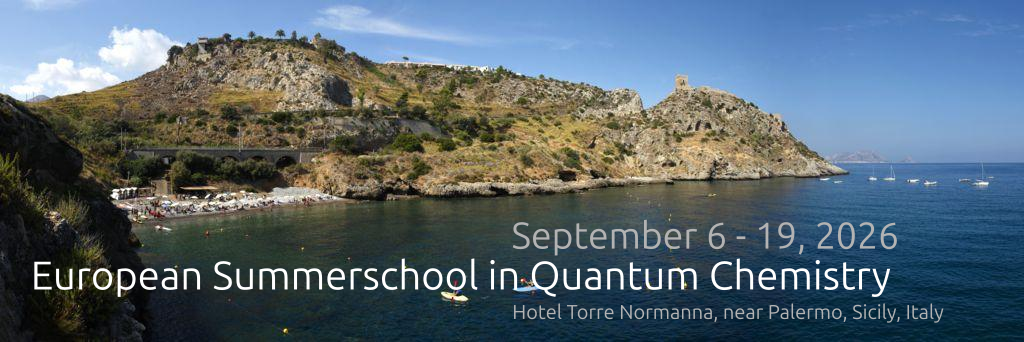
\includegraphics[width=0.7\textwidth]{fig/front}
%                \hspace{0.2\textwidth}
%                
\includegraphics[height=0.05\textwidth]{fig/CNRS}
        }
        
\begin{document}

%-----------------------------------------------------
%%%	TITLE		%%%
%-----------------------------------------------------
\begin{frame}
	\titlepage
\end{frame}

\begin{frame}{What's the idea?}
	\begin{equation}
		\boxed{\psi_p(\br) = \sum_\mu^K C_{\mu p} \phi_\mu(\br)}
	\end{equation}
	\begin{itemize}
		\item We want to approximate the orbitals as well as possible using basis functions
		\item We can use anything we want but we want to minimize $K$
		\item We also need to be able to compute one- and two-electron integrals
	\end{itemize}
\end{frame}

\begin{frame}{Basis functions are just legos!}
	\center
	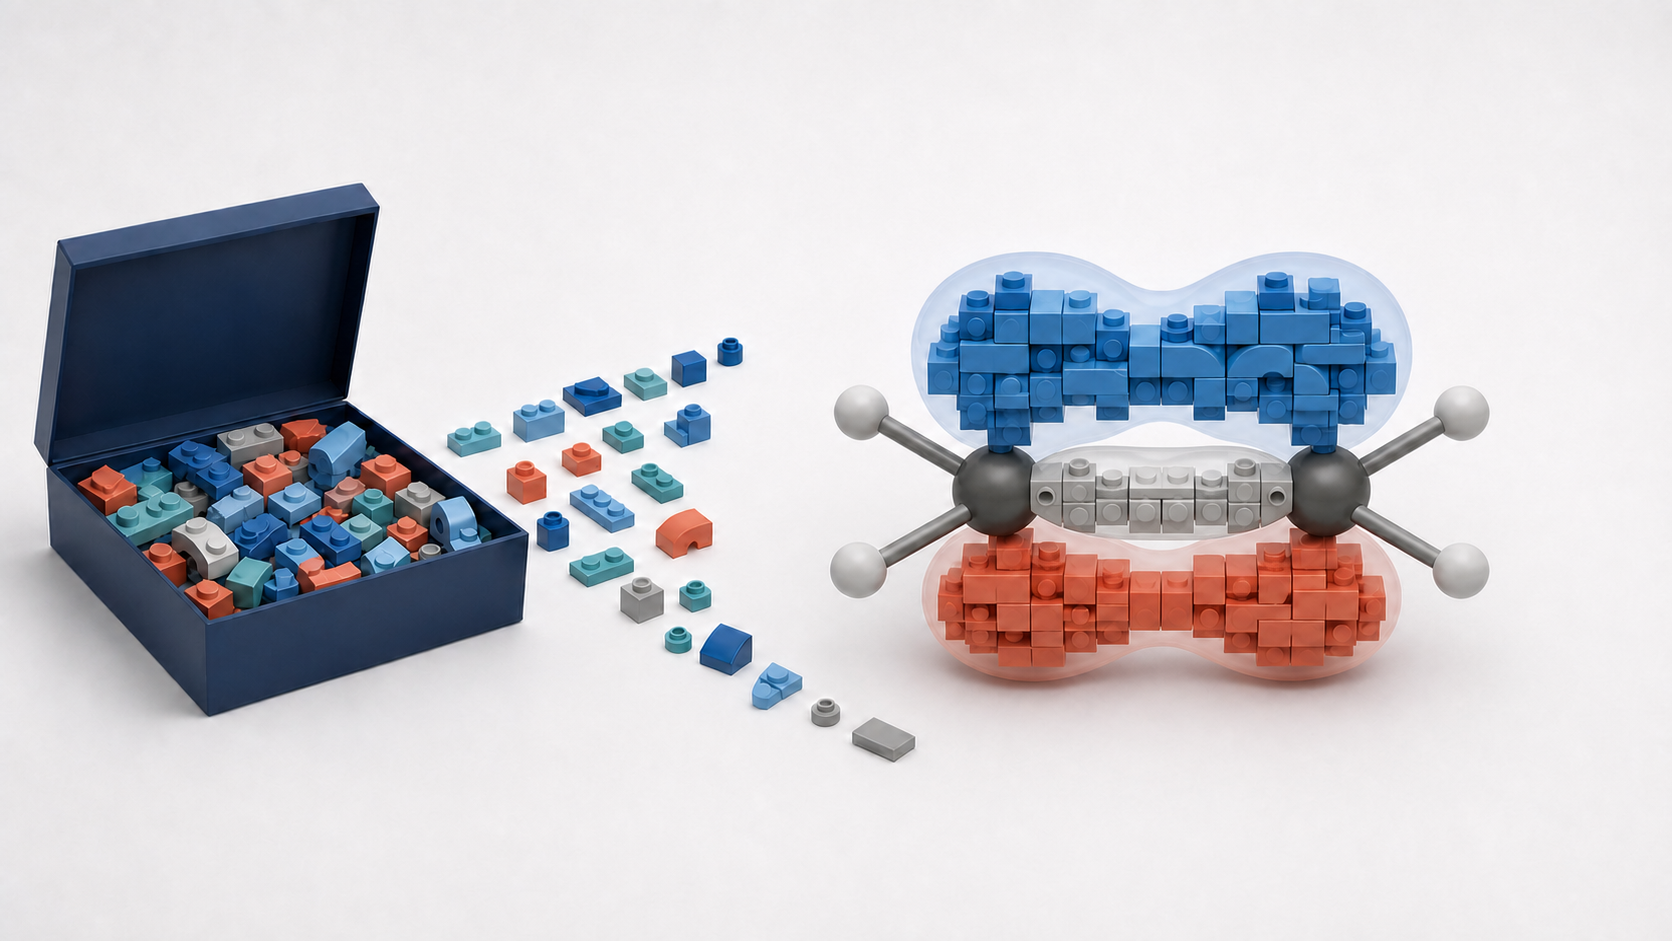
\includegraphics[width=0.9\textwidth]{fig/lego}
\end{frame}

\begin{frame}{Common basis functions}
	\begin{columns}
		\begin{column}{0.5\textwidth}
        	\begin{block}{Gaussian-type orbitals (GTOs)}
				\begin{equation}
					\phi(\br) = \exp(-\alpha r^2)
    			\end{equation}
    			\begin{itemize}
    				\item Usually atom-centered
    				\item Standard choice for molecular calculations
    				\item Efficient evaluation of multicenter integrals
    				\item Software: Orca, Q-Chem, Molcas, Molpro, PySCF, Psi4, CFOUR, MRCC, GAMESS, etc
    			\end{itemize}
        	\end{block}
        	\begin{block}{Slater-type orbitals (STOs)} 
				\begin{equation}
					\phi(\br) = \exp(-\zeta r)
        		\end{equation}
    			\begin{itemize}
    				\item Usually atom-centered
    				\item Natural nuclear cusp and exponential tail
    				\item Software: ADF
				\end{itemize}		
			\end{block}
		\end{column}
		\begin{column}{0.5\textwidth}
    		\begin{block}{Plane waves (PWs)}
				\begin{equation}
					\phi(\br) = \exp(\ii \bk \cdot \br)
				\end{equation}
    			\begin{itemize}
    				\item Delocalized and orthonormal
    				\item Naturally adapted to periodic systems
    				\item Systematically converged with an energy cutoff
    				\item Software: Quantum ESPRESSO, VASP, ABINIT, CASTEP, etc
    			\end{itemize}
			\end{block}
        	\begin{block}{Numerical atomic orbitals (NAOs)}
    			\begin{itemize}
    				\item Radial functions tabulated numerically
    				\item Compact and flexible atom-centered basis
    				\item Software: FHI-aims, SIESTA, etc
    			\end{itemize}
    		\end{block}
			\vspace{0.14\textwidth}
		\end{column}
	\end{columns}
\end{frame}

\begin{frame}{Plane waves}
	\begin{block}{Definition}
		\begin{equation}
			\phi_{\bk}(\br) = \frac{1}{\sqrt{\Omega}}\exp(\ii \bk \cdot \br)
			\qq{with}
			\abs{\bk} \le k_\text{cut}
			\qq{and} 
			E_\text{cut} = \frac{1}{2} k_\text{cut}^2
		\end{equation}
	\end{block}
	\begin{block}{Bloch wave vector}
		\begin{equation}
			\bk = k_1 \bb_1 + k_2 \bb_2 + k_3 \bb_3 
		\end{equation}
	\end{block}
	\begin{block}{Unit cell}
		\begin{equation}
			\underbrace{\Omega}_{\text{volume}} = \ba_1 \cdot (\ba_2 \cross \ba_3)
			\qq{with}
			\bA = (\ba_1,\ba_2,\ba_3)
		\end{equation}		
	\end{block}
	\begin{block}{Vectors of the reciprocal lattice}
		\begin{align}
			\bb_1 & = 2\pi \frac{\ba_2 \cross \ba_3}{\Omega}
			&
			\bb_2 & = 2\pi \frac{\ba_3 \cross \ba_1}{\Omega}
			&
			\bb_3 & = 2\pi \frac{\ba_1 \cross \ba_2}{\Omega}
		\end{align}		
	\end{block}
\end{frame}

\begin{frame}{Integrals in the plane wave basis}
	\begin{block}{Overlap integrals}
		\begin{equation}
			\braket{\bk_1}{\bk_2} 
			= \int \dd{\br} \phi_{\bk_1}^*(\br) \phi_{\bk_2}(\br)
			= \frac{1}{\Omega} \int \dd{\br} e^{\ii \qty( \bk_2 - \bk_1 ) \cdot \br}
			= \delta_{\bk_1 \bk_2}
			\qq{$\Rightarrow$}
			\alert{\text{Orthognal basis!}}
		\end{equation}
	\end{block}
	\begin{block}{Kinetic integrals}
		\begin{equation}
			\mel{\bk_1}{-\frac{\nabla^2}{2}}{\bk_2} 
			= \int \dd{\br} \phi_{\bk_1}^*(\br) \qty( - \frac{\nabla^2}{2}  ) \phi_{\bk_2}(\br)
			= \int \dd{\br} \phi_{\bk_1}^*(\br) \bk_2^2 \phi_{\bk_2}(\br)
			= \bk_2^2 \delta_{\bk_1 \bk_2}
			\qq{$\Rightarrow$}
			\alert{\text{Diagonal!}}
		\end{equation}
	\end{block}
	\begin{block}{Electron repulsion integrals}
		\begin{equation}
		\begin{split}
			\braket{\bk_1 \bk_2 }{\bk_3 \bk_4} 
			& = \iint \dd{\br_1} \dd{\br_2} \phi_{\bk_1}^*(\br_1) \phi_{\bk_2}^*(\br_2) r_{12}^{-1} \phi_{\bk_3}(\br_1) \phi_{\bk_4}(\br_2)
			\\
			& = \frac{1}{\Omega^2} \iint \dd{\br_1} \dd{\br_2} \frac{e^{\ii \qty( \bk_3 - \bk_1 ) \cdot \br_1} e^{\ii \qty( \bk_4 - \bk_2 ) \cdot \br_2}}{r_{12}}
		\end{split}
		\end{equation}
	\end{block}
\end{frame}

\begin{frame}{Resolution of the Coulomb operator}
	\begin{block}{Coulomb operator}
		\begin{equation}
			\frac{1}{r_{12}} 
			= \frac{1}{\Omega} \sum_{\bk \neq \bO} \frac{4\pi}{\bk^2} e^{\ii \bk \cdot (\br_1 - \br_2)}
		\end{equation}
		Dealing with the points where $\bk = \bO$ is a bit tricky bud doable...
	\end{block}

	\begin{block}{Electron repulsion integrals}
		\begin{equation}
		\begin{split}
			\braket{\bk_1 \bk_2 }{\bk_3 \bk_3} 
			& =  \frac{1}{\Omega^3} \sum_{\bk\neq\bO} \frac{4\pi}{\bk^2} \iint \dd{\br_1} \dd{\br_2} e^{\ii \qty( \bk_3 - \bk_1 - \bk ) \cdot \br_1} e^{\ii \qty( \bk_4 - \bk_2 +\bk) \cdot \br_2}
			\\
			& =  \frac{1}{\Omega} \sum_{\bk\neq\bO} \frac{4\pi}{\bk^2} \delta_{\bk_3-\bk_1-\bk,\bO} \delta_{\bk_4-\bk_2+\bk,\bO}
			\\
			& = \frac{4\pi}{\Omega \abs{\bk_1 - \bk_3}^2} \delta_{\bk_1+\bk_2,\bk_3+\bk_4}
			\qq{$\Rightarrow$}
			\alert{\text{Momentum conservation!}}
		\end{split}
		\end{equation}
	\end{block}
\end{frame}

\begin{frame}{Computing the electron repulsion integrals (ERIs)}
	\begin{columns}
		\begin{column}{0.7\textwidth}
			\begin{block}{Four-center two-electron integrals}
				\small
				\begin{equation}
					\begin{split} 
						\braket{\ba_1\ba_2}{\bb_1\bb_2}	
						& \equiv \mel{\ba_1\ba_2}{\alert{r_{12}^{-1}}}{\bb_1\bb_2}	
						\\
						& = \iint \phi_{\ba_1}^{\bA_1}(\br_1) \phi_{\ba_2}^{\bA_2}(\br_2) \,\alert{\frac{1}{r_{12}}}  \,
						\phi_{\bb_1}^{\bB_1}(\br_1) \phi_{\bb_2}^{\bB_2}(\br_2) \dd{\br_1} \dd{\br_2}
					\end{split}
				\end{equation}
				\alert{Formally, one has to compute $\order{N^4}$ ERIs!}
			\end{block}
		\end{column}
		\begin{column}{0.3\textwidth}
			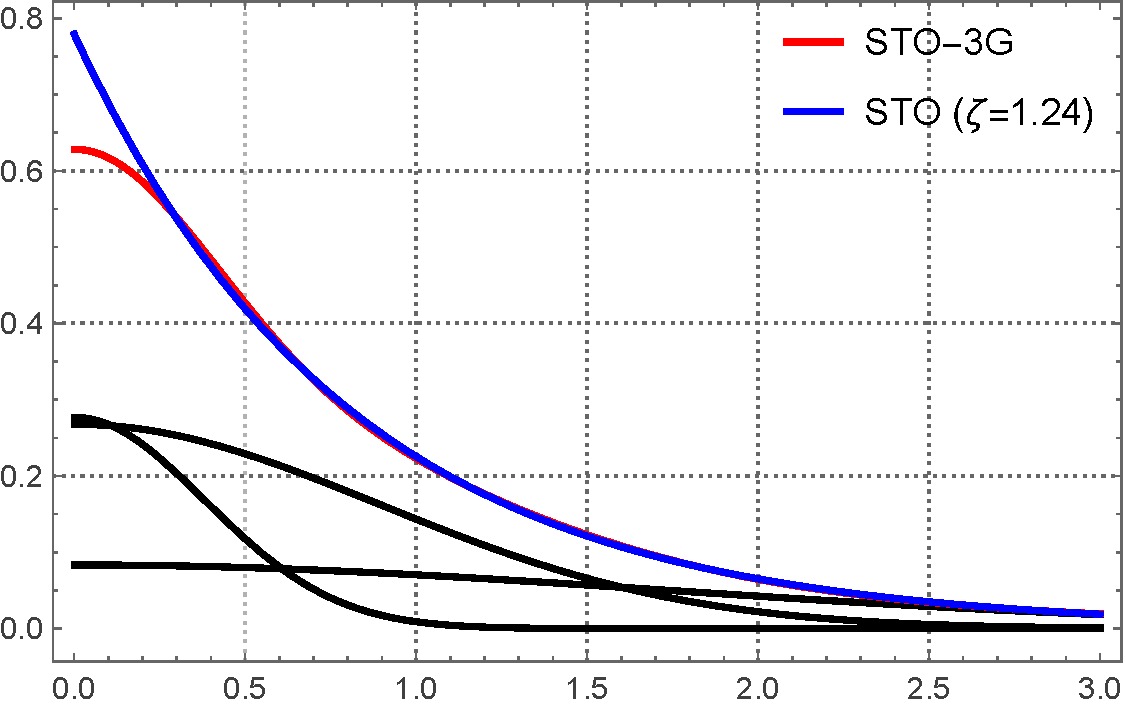
\includegraphics[width=\textwidth]{fig/STO}
		\end{column}
	\end{columns}
			%
			\begin{block}{Gaussian-type orbital (GTO)}
				\small
				\begin{align*} 
					\text{\violet{Contracted} GTO} & = \ket{\ba}
					\equiv \phi_{\ba}^{\bA}(\br)
					=  \sum_k^K D_k \sket{\ba}_k
					\\
					\text{\blue{Primitive} GTO} & =  \sket{\ba}
					=  (x-A_x)^{a_x} (y-A_y)^{a_y} (z-A_z)^{a_z} e^{-\alpha \abs{ \br -\bA }^2}
				\end{align*} 
			\end{block}
	\begin{itemize}
		\item \textbf{\purple{Exponent:}} $\alpha$
		\item \textbf{\purple{Center:}} $\bA = (A_x, A_y, A_z)$
		\item \textbf{\purple{Angular momentum:}} $\ba = (a_x, a_y, a_z)$ and total angular momentum $a=a_x + a_y + a_z$
	\end{itemize}
	%
\end{frame}

\begin{frame}{The contraction problem}
	\begin{columns}
		\begin{column}{0.7\textwidth}
			\begin{block}{Primitive vs Contracted}
				\begin{itemize}
					\item Same center $\bA$
					\item Same angular momentum $\ba$
					\item Different exponent $\violet{\alpha_k}$
					\item Contraction coefficient $\blue{D_k}$ and degree $K$
				\end{itemize}
				\begin{equation}
					\underbrace{\braket{\ba_1\ba_2}{\bb_1\bb_2}}_{\text{\green{contracted ERI}}} 
					= \sum_{k_1}^{K_1} \sum_{k_2}^{K_2} \sum_{k_3}^{K_3} \sum_{k_4}^{K_4} 
					\blue{D_{k_1} D_{k_2} D_{k_3} D_{k_4}}
					\underbrace{\sbraket{\ba_{1,k_1}\ba_{2,k_2}}{\bb_{1,k_3}\bb_{2,k_4}}}_{\text{\red{primitive ERI}}} 
				\end{equation}
				\centering
				\green{One} contracted ERI required \red{$K_1 \times K_2 \times K_3 \times K_4$} primitive ERIs!
			\end{block}
			\begin{block}{Dunning's cc-pVTZ basis for the carbon atom}
				\begin{equation}
					\green{\braket{1s1s}{1s1s}}
					= \sum_{k_1}^{10} \sum_{k_2}^{10} \sum_{k_3}^{10} \sum_{k_4}^{10} 
					\blue{D_{k_1} D_{k_2} D_{k_3} D_{k_4}}
					\red{\sbraket{s_{k_1}^{\violet{\alpha_{k_1}}} s_{k_2}^{\violet{\alpha_{k_2}}}} {s_{k_3}^{\violet{\alpha_{k_3}}} s_{k_4}^{\violet{\alpha_{k_4}}} }} 
				\end{equation}
				\centering
				The $\green{\braket{1s1s}{1s1s}}$ integral requires $10^4$ \red{$s$-type integrals}!
			\end{block}
		\end{column}
		\begin{column}{0.3\textwidth}
			\begin{equation}
				\boxed{\green{\ket{\ba}} = \sum_k^K \blue{D_k} \red{\sket{\ba_k}}}
			\end{equation}
			\\
			\bigskip
			\begin{block}{\small https://www.basissetexchange.org}
				\bigskip
				\centering
				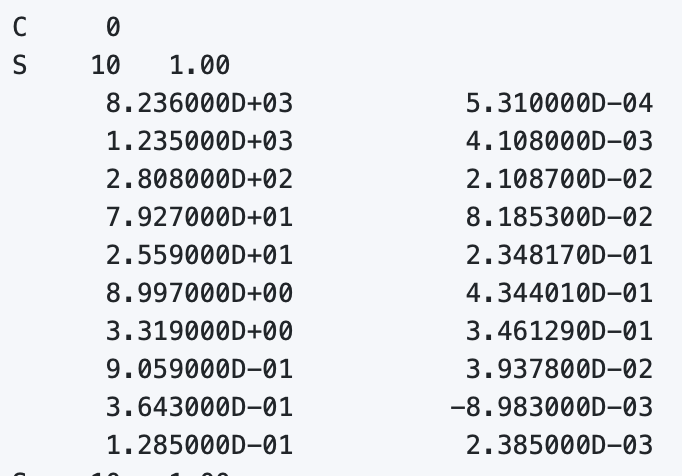
\includegraphics[width=\textwidth]{fig/C}
			\end{block}
		\end{column}
	\end{columns}
\end{frame}

%%% SLIDE X %%%
\begin{frame}{Properties of Gaussian functions}
	\begin{block}{Gaussian product rule: \textit{``The product of two gaussians is a gaussian''}}
		\begin{equation}
			G_{\red{\alpha},\red{\bm{A}}}(\br) = \exp(-\red{\alpha} \abs{\br - \red{\bA}}^2)	
			\qqtext{and}
			G_{\blue{\beta},\blue{\bm{B}}}(\br) = \exp(-\blue{\beta} \abs{\br - \blue{\bB}}^2)	
			\qqtext{then}
		\end{equation}	
		\begin{equation}
		\boxed{G_{\red{\alpha},\red{\bm{A}}}(\br) G_{\blue{\beta},\blue{\bm{B}}}(\br) = \violet{K} \, G_{\violet{\zeta},\violet{\bm{P}}}(\br)}
		\qqtext{with} 
		\violet{\zeta} = \red{\alpha} + \blue{\beta} 
		\qqtext{and} 
		\violet{\bm{P}} = \frac{\red{\alpha \bA} + \blue{\beta \bB}}{\red{\alpha} + \blue{\beta} } 
		\end{equation}		
		\begin{equation}
			\violet{K_{\zeta,\bm{P}}} = \exp( -\frac{\red{\alpha} \blue{\beta}}{\red{\alpha} + \blue{\beta} } \abs{\red{\bA} - \blue{\bB}}^2)
		\end{equation}		
	\end{block}
	\begin{block}{Gaussian product rule for ERIs}
		\begin{equation}
			\begin{split}
			(\bm{\red{a}} \bm{\blue{b}}|\bm{\orange{c}} \bm{\green{d}}) 
			& = \iint  \dd{\br_1} \dd{\br_2} G_{\red{\alpha},\red{\bm{A}}}(\br_1) G_{\blue{\beta},\blue{\bm{B}}}(\br_1) \frac{1}{r_{12}} G_{\orange{\gamma},\orange{\bm{C}}}(\br_2) G_{\green{\delta},\green{\bm{D}}}(\br_2)
			\\
			& = \violet{K_{\zeta,\bm{P}}} \violet{K_{\eta,\bm{Q}}} \iint \dd{\br_1} \dd{\br_2} G_{\violet{\zeta},\violet{\bm{P}}}(\br_1) \frac{1}{r_{12}} G_{\purple{\eta},\purple{\bm{Q}}}(\br_2) 
		\end{split}	
		\end{equation}	
		\alert{The number of ``significant'' ERIs in a large system is $\order{N^2}$!}
	\end{block}
\end{frame}
%

\begin{frame}{Upper bounds for ERIs}
	\begin{columns}
		\begin{column}{0.4\textwidth}
			\begin{block}{A ``good'' upper bound must be}
				\begin{itemize}
					\item simple, i.e, cheap to compute
					\item strong, i.e., a good estimate
					\item scaling-consistent, i.e., $N_\text{sig} = \order*{N_\text{upper}}$
				\end{itemize}
			\end{block}
		\end{column}
		\begin{column}{0.6\textwidth}
    		\begin{equation}
    			\boxed{\abs{(\bm{\red{a}} \bm{\blue{b}}|\bm{\orange{c}} \bm{\green{d}})} \le B}
    		\end{equation}
    		\begin{itemize}
    			\item $(\bm{\red{a}} \bm{\blue{b}}|$ = single bra and $(\red{a} \blue{b}|$ = shell-pair 
    			\item $(\bm{\red{a}} \bm{\blue{b}}|\bm{\orange{c}} \bm{\green{d}})$ = single integral and $(\red{a} \blue{b}|\orange{c} \green{d})$ = shell-quartet 
    		\end{itemize}
		\end{column}
	\end{columns}
	\bigskip
	\begin{block}{Cauchy-Schwartz bound}
		\begin{equation}
			\abs{(\bm{\red{a}} \bm{\blue{b}}|\bm{\orange{c}} \bm{\green{d}})} 
			\le 
			\sqrt{(\bm{\red{a}} \bm{\blue{b}}|\bm{\red{a}} \bm{\blue{b}})} 
			\sqrt{(\bm{\orange{c}} \bm{\green{d}}|\bm{\orange{c}} \bm{\green{d}})}
			\qqtext{or}
			\abs{(\bm{\violet{P}}|\bm{\purple{Q}})} 
			\le 
			\sqrt{(\bm{\violet{P}}|\bm{\violet{P}})} 
			\sqrt{(\bm{\purple{Q}}|\bm{\purple{Q}})}
		\end{equation}
	\end{block}
	\begin{block}{The family of generalized H\"older bounds}
		\begin{equation}
			\abs{(\bm{\red{a}} \bm{\blue{b}}|\bm{\orange{c}} \bm{\green{d}})} 
			\le 
			\qty[ (\bm{\red{a}} \bm{\blue{b}}|\bm{\red{a}} \bm{\blue{b}}) ]^{1/\purple{m}} 
			\qty[ (\bm{\orange{c}} \bm{\green{d}}|\bm{\orange{c}} \bm{\green{d}}) ]^{1/\violet{n}}
			\qqtext{with}
			\frac{1}{\purple{m}} + \frac{1}{\violet{n}} = 1
			\qqtext{and}
			\purple{m},\violet{n} > 1
		\end{equation}
	\end{block}
\end{frame}

\begin{frame}{Cauchy-Schwartz bound}
	\begin{equation}
		(\bm{\red{a}} \bm{\blue{b}}|\bm{\orange{c}} \bm{\green{d}})
		= (\bm{\violet{P}}|\bm{\violet{Q}})
		\le 
		\sqrt{(\bm{\violet{P}}|\bm{\violet{P}})} 
		\sqrt{(\bm{\purple{Q}}|\bm{\purple{Q}})}
	\end{equation}
	\begin{itemize}
		\item $(\bm{\violet{P}}|\bm{\violet{Q}})$ should decay as $1/\abs{\violet{\bm{P}} - \violet{\bm{Q}}}$ or faster
		\item However, there is no distance information in the product $(\bm{\violet{P}}|\bm{\violet{P}}) (\bm{\violet{Q}}|\bm{\violet{Q}})$
		\item The Cauchy-Schwarz bound is rigorous and cheap but is not tight for well-separated shell pairs.
	\end{itemize}
\end{frame}


\begin{frame}{A tale of three strategies}
\begin{itemize}
	\item \orange{\bf Integral bound}
		\\
		We seek a single number that bounds a particular integral
		\begin{equation*}
			\abs{\sbraket{\ba_1\ba_2}{\bb_1\bb_2}} \le \sbraket{\ba_1\ba_1}{\bb_1\bb_1}^{1/2} \sbraket{\ba_2\ba_2}{\bb_2\bb_2}^{1/2}
		\end{equation*}
		With $\order{N^{2}}$ $\sbraket{\ba_1\ba_1}{\bb_1\bb_1}$ bound factors, we can upper bound $\order{N^{4}}$ $\sbraket{\ba_1\ba_2}{\bb_1\bb_2}$ integrals

	\item \alert{\bf Non-factorizable class bound}
		\\
		We seek a single number that bounds an entire class*
		\begin{equation*}
			\abs{\sbraket{a_1a_2}{b_1b_2}} \le \sbraket{\sba_{1} \sba_{2}}{\sbb_{1} \sbb_{2}}
		\end{equation*}
	\item \violet{\bf Factorizable class bound}
		\\
		We combine the two previous ideas
		\begin{equation*}
			\begin{split}
				\left| \sbraket{a_1a_2}{b_1b_2}  \right| 
				& \le \sbraket{\sba_{1} \sba_{2}}{\sbb_{1} \sbb_{2}}
				\\
				& \le \sbraket{\sba_1\sba_1}{\sbb_1\sbb_1}^{1/2} \sbraket{\sba_2\sba_2}{\sbb_2\sbb_2}^{1/2}
			\end{split}
		\end{equation*}
\end{itemize}
*{\small The simple $\sbraket{dd}{dd}$ class is made of 625 integrals!}
\end{frame}


\begin{frame}{Asymptotic scaling of two-electron integrals}
	\begin{block}{Number of significant two-electron integrals}
		\begin{equation}
			(\bm{\red{a}} \bm{\blue{b}}|\bm{\orange{c}} \bm{\green{d}}) \equiv (\bm{\red{a}} \bm{\blue{b}}| \mathcal{O}_2 | \bm{\orange{c}} \bm{\green{d}})
		\end{equation}
	\end{block}
	\bigskip
	\begin{block}{Long-range vs short-range operators}
		\begin{equation}
			N_\text{sig} =  c\,N^{\alpha}
		\end{equation}
		\center
		\begin{tabular}{lcrccrc}
			\hline
			\hline
			Molecule			& 	$N$ 	& 	\mc{2}{c}{\red{$\hO = r_{12}^{-1}$}} 		&& 	\mc{2}{c}{\orange{$\hO = e^{-r_{12}^2}$}} 		 	\\
										\cline{3-4}								\cline{6-7}					
							& 		& 	\mc{1}{c}{$N_\text{sig}$}	& $\alpha$ 	&& 	\mc{1}{c}{$N_\text{sig}$}	& $\alpha$ 	 \\
			\hline
			propene			&	12	&	1\,625		&	---		&&	1\,650		&	---			\\
			butadiene			&	16	&	5\,020		&	3.9		&&	5\,020		&	3.9			\\
			hexatriene			&	24	&	24\,034		&	3.9		&&	23\,670		&	3.8			\\
			octatetraene		&	32	&	63\,818		&	3.4		&&	52\,808		&	2.8			\\
			decapentaene		&	40	&	119\,948		&	2.8		&&	81\,404		&	1.9			\\
			dodecaexaene		& 	48	&	192\,059		&	2.6		&&	109\,965		&	1.6			\\
			\hline
			\hline
		\end{tabular}
		\bigskip
	\end{block}
\end{frame}


\begin{frame}{Recipe for computing two-electron integrals}
\center
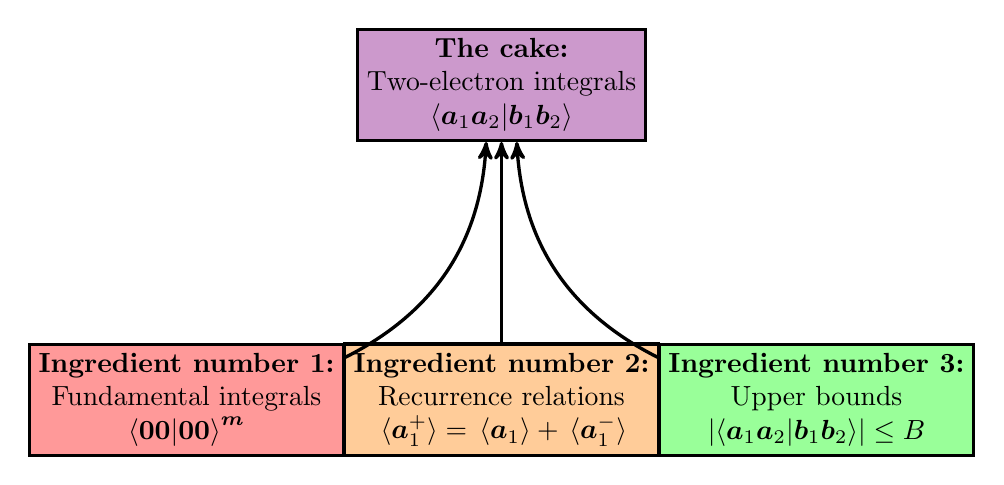
\begin{tikzpicture}
	\begin{scope}[very thick,
		node distance=4cm,on grid,>=stealth',
		boxRR/.style={rectangle,draw,fill=green!40},
		boxUB/.style={rectangle,draw,fill=orange!40},
		boxFI/.style={rectangle,draw,fill=red!40},
		integral/.style={rectangle,draw,fill=violet!40}],
		\node [integral, align=center]		(1)					{\textbf{The cake:} \\ Two-electron integrals \\ $\braket{\ba_1 \ba_2}{ \bb_1 \bb_2}$};
		\node [boxUB, align=center]		(2A)		[below=of 1]	{\textbf{Ingredient number 2:} \\ Recurrence relations \\ $\expval*{\ba_1^+} = \expval*{\ba_1} + \expval*{\ba_1^-}$};
		\node [boxRR, align=center] 		(2B)		[right=of 2A]	{\textbf{Ingredient number 3:} \\ Upper bounds \\ $\abs{\braket{\ba_1 \ba_2}{ \bb_1 \bb_2}} \le B$};
		\node [boxFI, align=center]		(2C)		[left=of 2A]	{\textbf{Ingredient number 1:} \\ Fundamental integrals \\ $\braket{\bO\bO}{\bO\bO}^{\bm{m}}$};
		\path 
		(1) edge [<-]			(2A)
		(1) edge [<-,bend right]			(2B)
		(1) edge [<-,bend left]					(2C)
		;
	\end{scope}
\end{tikzpicture}
\end{frame}

\begin{frame}{Late-contraction path algorithm (Head-Gordon-Pople \& PRISM inspired)}
	\begin{tikzpicture}
		\begin{scope}[
			very thick,
			node distance=1.5cm,on grid,>=stealth',
			boxSP/.style={rectangle,draw,fill=purple!40},
			box0m/.style={rectangle,draw,fill=red!40},
			boxCm/.style={rectangle,draw,fill=gray!40},
			boxA/.style={rectangle,draw,fill=red!40},
			boxAA/.style={rectangle,draw,fill=red!40},
			boxAAA/.style={rectangle,draw,fill=red!40},
			boxC/.style={rectangle,draw,fill=gray!40},
			boxCC/.style={rectangle,draw,fill=gray!40},
			boxCCC/.style={rectangle,draw,fill=orange!40},
			boxCCCCCC/.style={rectangle,draw,fill=green!40},
			],
			\node [boxSP, align=center]			(SP)									{Shell-pair \\ data};
			\node [box0m, align=center]			(0m)			[right=of 1,xshift=1.25cm]		{$\sbraket{00}{00}^{\bm{m}}$};
			\node [boxCm, align=center]			(Cm)			[right=of 0m,xshift=1.75cm]	{$\braket{00}{00}^{\bm{m}}$};
			\node [boxA, align=center] 			(A)			[below=of 0m]				{$\sbraket{0 a_2}{00}^{\bm{m}}$};
			\node [boxC, align=center] 			(C)			[right=of A,xshift=1.75cm]		{$\braket{0 a_2}{00}^{\bm{m}}$};
			\node [boxAA, align=center] 			(AA)			[below=of A]				{$\sbraket{a_1 a_2}{00}$};
			\node [boxCC, align=center] 			(CC)			[right=of AA,xshift=1.75cm]	{$\braket{a_1 a_2}{00}$};
			\node [boxCCCCCC, align=center] 		(CCCC)	[right=of CC,xshift=2cm]		{$\braket{a_1 a_2}{b_1 b_2}$};
			\path 
			(SP)		edge[->]			node[below,blue]{T$_0$}									(0m)
			(0m)		edge[->]			node[left,orange]{T$_1$}			node [right,red]{VRR$_1$}	(A)
			(0m)		edge[->,gray!70]														(Cm)
			(A)		edge[->]			node[left,orange]{T$_2$}			node [right,red]{VRR$_2$}	(AA)
			(A)		edge[->,gray!70]														(C)
			(AA)		edge[->]			node [below,blue]{CC}											(CC)
			(Cm)		edge[->,gray!70]														(C)
			(C)		edge[->,gray!70]														(CC)
			(CC)	edge[->]			node [above,orange]{T$_3$}		node [below,red]{HRR}		(CCCC)
			;
		\end{scope}
	\end{tikzpicture}
	\bigskip
	\begin{itemize}
		\item \red{HRR} = horizontal recurrence relation [Obara-Saika]
		\item \red{VRR} = vertical recurrence relation
		\item \blue{CC} = bra contraction
	\end{itemize}
\end{frame}

\begin{frame}{Computing the fundamental integrals}
	\begin{equation}
		\sbraket{\bO\bO}{\bO\bO}^{\bm{m}} 
		\equiv (\bm{\red{a}} \bm{\blue{b}}|\bm{\orange{c}} \bm{\green{d}})
		= (\bm{\violet{P}}|\bm{\violet{Q}})
	\end{equation}
	\begin{block}{Shell-pair data}
		\begin{equation}
			\bR = \bQ - \bP
			2\vartheta = 1/(
		\end{equation}
	\end{block}
	\begin{block}{Shell-pair data}
		\begin{equation}
			\sbraket{\bO\bO}{\bO\bO}^{\bm{m}} = U (2\theta^2)^{m+1/2} G_m(T)
		\end{equation}
		\begin{equation}
			G_m(T) = \qty( \frac{2}{\pi} )^{1/2} \int_0^1 t^{2m} \exp(-T t^2) \dd{t}
		\end{equation}
		it can be efficiently evaluated by Chebyshev interpolation.
	\end{block}	
\end{frame}

\begin{frame}{Recurrence relations}
	\begin{block}{Vertical recurrence relation}
	\end{block}
	\begin{block}{Horizontal recurrence relation}
	\end{block}	
\end{frame}


%\begin{frame}{Screening algorithm for two-electron integrals}
%
%\resizebox{\textwidth}{!}{
%\begin{tikzpicture}
%	\begin{scope}[very thick,
%		node distance=2.5cm,on grid,>=stealth',
%		bound2/.style={diamond,draw,fill=blue!40},
%		bound4/.style={diamond,draw,fill=blue!40},
%		bound6/.style={diamond,draw,fill=blue!40},
%		shell/.style={circle,draw,fill=green!40},
%		shellpair/.style={circle,draw,fill=green!40},
%		shellquartet/.style={circle,draw,fill=green!40},
%		shell1/.style={rectangle,draw,fill=yellow!40},
%		shell2/.style={rectangle,draw,fill=orange!40},
%		shell3/.style={rectangle,draw,fill=red!40},
%		integral/.style={rectangle,draw,fill=violet!40}],
%		\node [shell1, align=center]		(1)											{Primitive\\shells\\$\sket{a}$};
%		\node [bound2, align=center] 		(B2)			[right=of 1]				{$\sexpval{B_2}$};
%		\node [shell, align=center]			(S1T)		[above=of B2, yshift=-0.5cm]	{$\sket{a}$};
%		\node [shell, align=center]			(S1B)		[below=of B2, yshift=0.5cm]		{$\sket{b}$};
%		\node [shell2, align=center] 		(2)			[right=of B2,xshift=0.75cm]		{Contracted\\shell-pairs\\$\ket{ab}$};
%		\node [bound4, align=center]		(B4)			[right=of 2]				{$\expval{B_4}$} ;
%		\node [shellpair, align=center]		(S2T)		[above=of B4, yshift=-0.5cm]	{$\ket{a_1b_1}$};
%		\node [shellpair, align=center]		(S2B)		[below=of B4, yshift=0.5cm]		{$\ket{a_2b_2}$};
%		\node [shell3, align=center]		(3)			[right=of B4]					{Two-Electron\\integrals\\$\braket{a_1b_1}{a_2b_2}$};
%		\path 
%		(1) edge [->,bend left]				(S1T)
%		(1) edge [->,bend right]			(S1B)
%		(S1T) edge [snake it]				(B2)
%		(S1B) edge [snake it]				(B2)
%		(B2) edge [->,color=red] 	node [below] {\small Contraction}		(2)
%		(2) edge [->,bend left] 				(S2T)
%		(2) edge [->,bend right] 			(S2B)
%		(S2T) edge [snake it]				(B4)
%		(S2B) edge [snake it]				(B4)
%		(B4) edge [->] 					(3)
%		;
%	\end{scope}
%\end{tikzpicture}
%}
%\end{frame}


\end{document}
